Другой метод предложенный авторами работы \cite{piezo50} заключается в измерении интенсивности для разной
отстройки от точного брэговского угла кристалла образца в двухкристальной схеме дифрактометра.
Необходимо  встать в произвольную точку на кривой дифракционного отражения,
другими словами выведем интенсивность детектора из максимума отражения в точку на склоне
 кривой (Рис.~\ref{ris:kdopiez}).

\begin{figure}[H]
\centering
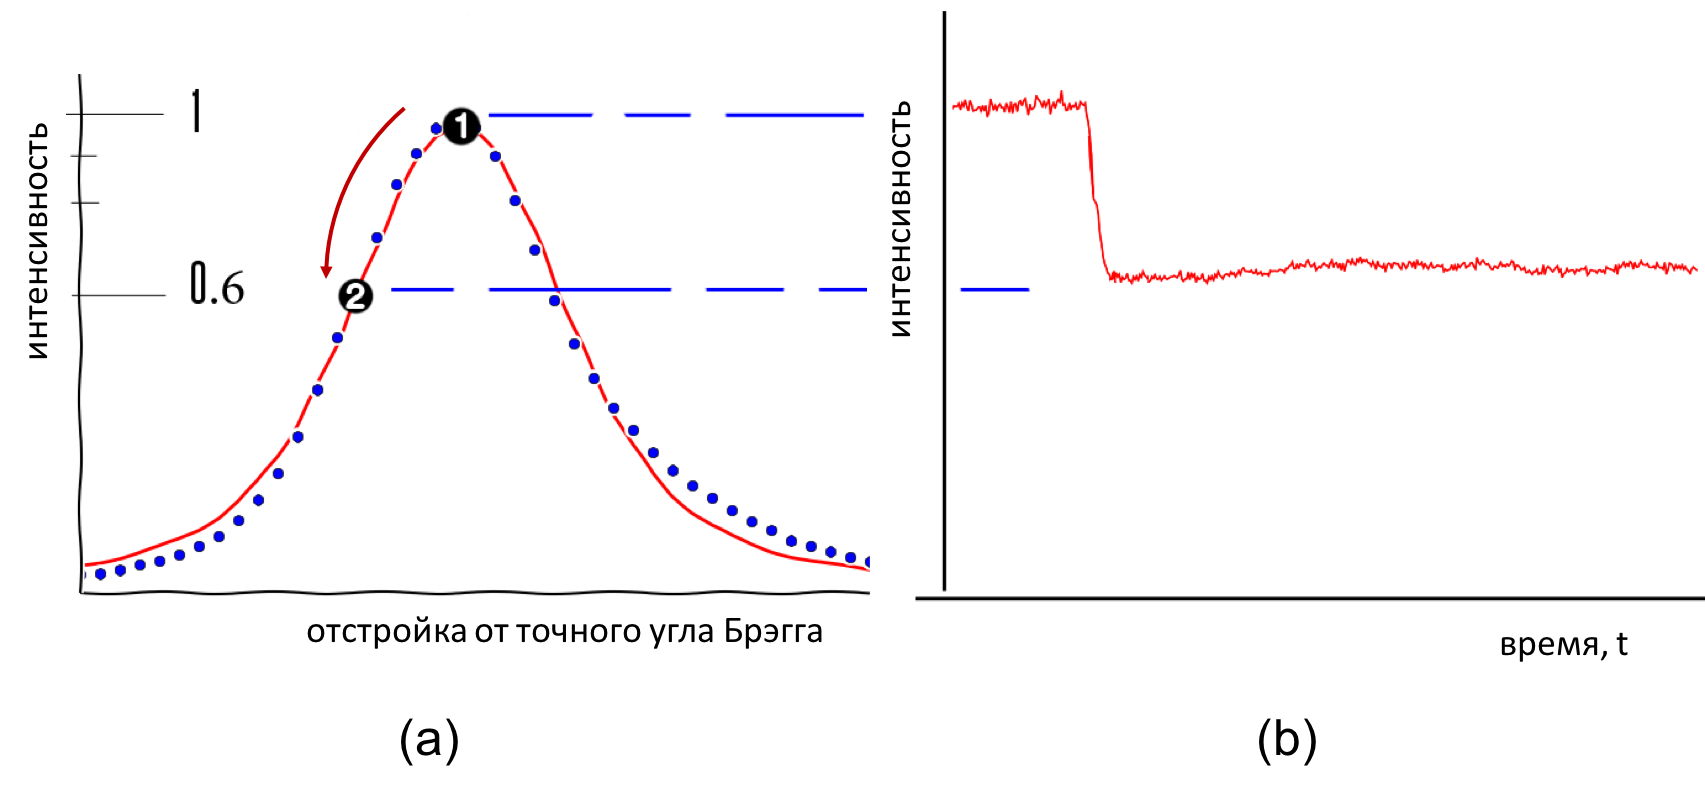
\includegraphics[width=1\linewidth]{images/kdopiez2.png}
\caption{Смещение точки на КДО (a), интенсивность сигнала на детекторе (b)}
\label{ris:kdopiez}
\end{figure}

При включении электрического поля (рис. \ref{ris:princip}b) для разных направлений наблюдаем изменение интенсивности
на детекторе (рис. \ref{ris:princip}a). Изменение интенсивности характеризует динамику смещения
двухкристальной КДО (рис. \ref{ris:princip}с) вследствие изменения межплоскостного расстояния в образце.

\begin{figure}[H]
\centering
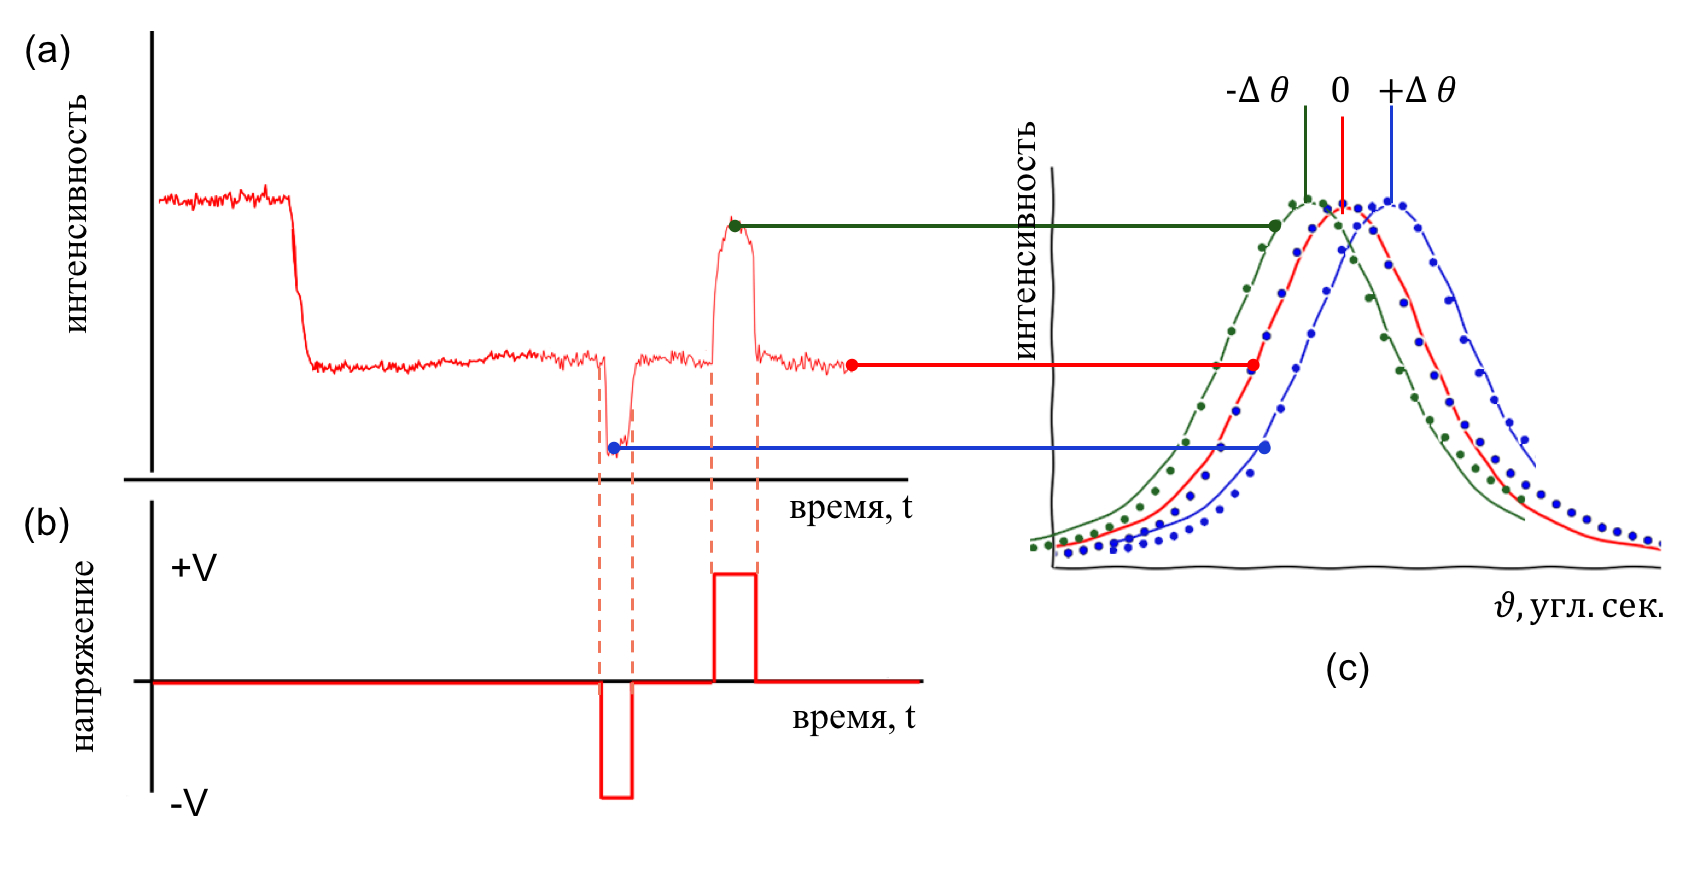
\includegraphics[width=0.8\linewidth]{images/princip2.png}
\caption{Интенсивность сигнала на детекторе (a); (b) величина  приложенного напряжения к
поверхности кристалла; (c) восстановленное положение КДО  }
\label{ris:princip}
\end{figure}

Данный метод является наиболее быстрым, т.к. изменение интенсивности на детекторе происходит практически сразу (за время порядка - мс.),
из рис. \ref{ris:princip}  видно, что время за которое деформируется кристалл много меньше разрешающей способности метода.
Данная методика применима в том случае, если КДО полученная от кристалла - пьезоэлектрика, под воздействием электрического поля,
остается постоянной.

% Но дальше будет показано, что наряду с пьезоэлектрическим эффектом могут присутствовать и сопровождающие
% процессы, которые ведут к не мгновенному смещению, а протекают за конечное время.

  %
  % Горфман \cite{piezo51} усовершенствовал данную методику, добавив схему совпадения, которая позволяет
  % снимать двухкристальную кривую классическим методом с увеличенной временной задержкой в каждой точке отстройки.
  % Увеличение времени необходимо для измерения интенсивность до момента подачи поля и после включения
  %  электрического поля, включение которого согласуется с помощью высокочастотного анализатора с детектором.
